\documentclass{emulateapj}
\submitted{{\it Submitted for publication in ApJL}}
\usepackage{multirow,color,wrapfig,ulem}
\usepackage {graphicx}

\usepackage{graphics}
\usepackage[dvips]{epsfig}

\newcommand{\lcdm}{$\Lambda$CDM }
\newcommand{\mpc}{\rm{Mpc}}
\newcommand{\avg}[1]{\langle{#1}\rangle}  
\newcommand{\nscatt}{\langle N_{\rm  scatt}\rangle}
\newcommand{\ly}{{\ifmmode{{\rm Ly}\alpha~}\else{Ly$\alpha$~}\fi}}
\newcommand{\hMpc}{{\ifmmode{h^{-1}{\rm Mpc}}\else{$h^{-1}$Mpc }\fi}}   
\newcommand{\hGpc}{{\ifmmode{h^{-1}{\rm Gpc}}\else{$h^{-1}$Gpc }\fi}}   
\newcommand{\hmpc}{{\ifmmode{h^{-1}{\rm Mpc}}\else{$h^{-1}$Mpc }\fi}}  
\newcommand{\hkpc}{{\ifmmode{h^{-1}{\rm kpc}}\else{$h^{-1}$kpc }\fi}}  
\newcommand{\hMsun}{{\ifmmode{h^{-1}{\rm
        {M_{\odot}}}}\else{$h^{-1}{\rm{M_{\odot}}}$}\fi}}   
\newcommand{\hmsun}{{\ifmmode{h^{-1}{\rm
        {M_{\odot}}}}\else{$h^{-1}{\rm{M_{\odot}}}$}\fi}}   
\newcommand{\Msun}{{\ifmmode{{\rm {M_{\odot}}}}\else{${\rm{M_{\odot}}}$}\fi}}  
\newcommand{\msun}{{\ifmmode{{\rm {M_{\odot}}}}\else{${\rm{M_{\odot}}}$}\fi}}  
\newcommand{\lya}{{Lyman$\alpha$~}}
\newcommand{\clara}{{\texttt{CLARA}}~}
\newcommand{\rand}{{\ifmmode{{\mathcal{R}}}\else{${\mathcal{R}}$ }\fi}}  
\newcommand{\hs}{{\hspace{1mm}}}  
\newcommand{\kms}{{\ifmmode{{\mathrm{\,km\ s}^{-1}}}\else{\,km~s$^{-1}$}\fi}}

% definition to produce a "less than or similar to" symbol
\def\lsim{~\rlap{$<$}{\lower 1.0ex\hbox{$\sim$}}}

% definition to produce a "greater than or similar to" symbol
\def\gsim{~\rlap{$>$}{\lower 1.0ex\hbox{$\sim$}}}

\begin{document}

\title{The Place of the Local Group in the Cosmic Web} 
\author{
  XXXX\altaffilmark{1},
  YYYY\altaffilmark{2},
  ZZZZ\altaffilmark{3}
}

\altaffiltext{1}{Uni A}
\altaffiltext{2}{Uni B}
\altaffiltext{3}{Uni C}
\begin{abstract}
This
\end{abstract}

\begin{keywords}
{galaxies: Local Group --- dark matter}
\end{keywords}


\section{Introduction}
\label{sec:intro}

%lg rare
The configuration of galaxies in the Local Group (LG hereafter) is quite rare to find in the local Universe and in cosmological simulations. 
The LG is dominated by the two big spirals MW and M31, the next most-luminous galaxy is M33 which is $\sim 10$ times less massive than M31, followed by several less luminous dwarf galaxies, up to a distance of $\sim 3$\mpc.
The velocity vector of M31, with a low tangential velocity is
consistent to a head-on collision orbit toward the MW
\citep{2008MNRAS.386..461C,2012ApJ...753....8V,2012ApJ...753....7S}. 

Another feature of the Local group is the relatively low velocity
dispersion of nearby galaxies up to $\sim 8$ Mpc \citep[][and
  references therein]{1975ApJ...196..313S,2011MNRAS.415L..16A}. 
Environment around the Local Group has density quite close to the
average density of the universe
\citep{2003ApJ...596...19K,2005AJ....129..178K}. In addition, the
closest massive galaxy cluster, the Virgo Cluster, is $\approx
16.5\ \mpc$ away \citep{2007ApJ...655..144M}. 

All this combination of features make LG analogues very rare to
find. Using numerical simulatons \citet{lganalogues} found less than
$2\%$ MW-sized halos reside in a pair similar to MW-M31 and in a
similar environment. Furthermore, if we select pairs constrained
within $2\sigma$ error fron current observational measurements of the
velocity components and distance to M31, there are only $88$ systems
in a cube of $250$ \hmpc side. 

\citet{2013ApJ...767L...5F} also study MW-M31 pairs in numerical
simulations finding the typical quantities characterizing the orbital
parameters of the LG are rare among typical pairs, but not enough to
challenge the \lcdm model. 
Another definition of LG analogues is made by
\citet{2008MNRAS.384.1459L}, but despite differences ocurr in the
definitions and resulting fraction of LG analogues, all are in
agreement with a low frequency of these pairs. 
%lw08 also look lg analogues

%larger scales & lg env
To understand better the properties of the LG and how this uncommon
pair configuration fit in the cosmological context, an immediate
question arise. What else can we say of the LG at larger scales?. In
particular, which are the typical/prefered locations of these systems
within the Cosmic Web?.

Looking the LG at larger scales we have it is located in a difuse and
warped filament/wall conecting Virgo Cluster with Fornax Cluster, some
nearby galaxies and groups members of this large structure are the
Maffei group, NGC $6744$, NGC $5128$, $M101$, $M81$, $NGC1023$, Cen A
group. At this scale, there is no evident alignment of the MW-M31
orbital plane with the local filament or the Virgo-Fornax direction.  

However, if we look in a smaller volume below scales of $\sim 6$ \mpc,
there is a clear alignment of th the MW-M31 orbit with a local plane
as shown by figure $3$ in \citet{2013AJ....146...69C}. 

%this paper.
In this paper we will study the large scale environment of LG
analogues using the Bolshoi simulation, in particular which kind of
structures they reside and if there is any correlation or alignment
with the cosmic web.  
Environment is defined by the cosmic web components identified by
\citet{Tweb}, and we use the LG analogues computed by
\citet{lganalogues}. 

Paper is organized ...


\section{Simulation and web finding algorithm}
\label{sec:Simulation}

\subsection{The Bolshoi simulation}
We use the Bolshoi simulation of $\Lambda$CDM cosmology: $\Omega_{\rm
  m}=1-\Omega_{\Lambda}=0.27$, $H_0=70\,\rm km/s/Mpc$,
$\sigma_8=0.82$, $n_s=0.95$ \citep{2011ApJ...740..102K}, compatible
with the constraints from the WMAP satellite
\citep{hinshaw_etal13}. The simulation followed evolution of dark
matter in a $250 \hmpc$ box with spatial resolution of $\approx
1h^{-1}$~kpc and mass resolution of $m_{\rm p}=1.35\times 10^8\ \rm
M_{\odot}$. Halos are identified with the BDM algorithm
\citep{1997astro.ph.12217K}. The BDM algorithm is  a spherical
overdensity halo finding algorithm and is designed to identify both
host halos and subhalos. 



\subsection{Cosmic web identification}
The web finding algorithm is based on the tidal tensor computed as the
Hessian of the  gravitational potential field

\begin{equation}
T_{ij} = \frac{\partial^2 \phi}{\partial r_i \partial r_j}, 
\end{equation}
where $r_{i}$, $i=1,2,3$ refers to the three spatial comoving
coordiates and $\phi$ is the gravitational potential renormalized to
follow the following Poisson equation $\nabla\phi=\delta$ where
$\delta$ is the matter overdensity.  

This tensor is real and symmetric, which means that can be
diagonalized. We note the eigenvalues $\lambda_1\geq \lambda_2\geq
\lambda_3$ and their corresponding eigenvectors $\hat{e}_1$,
$\hat{e}_2$ and $\hat{e}_3$. The web classification compares each one
of the three eigenvalues to a threshold value $\lambda_{\rm th}$. If the three, two, one or zero eigenvalues are larger than this threshold the region es classified as peak, filament, sheet or void, respectively. 

In \cite{Tweb} we perform a detailed study for the topology of the
cosmic web and its visual counterpart as a function of the parameter
$\lambda_{\rm th}$. We find that reasonable results in terms of the
volume fraction occupied by voids, the visual inspection and the halo
populations in each web type can be reached by values of $0.2<\lambda_{\rm
th}<0.4$. In this paper we choose the value of $\lambda_{\rm
  th}=0.3$. We have veryfied that the main trends reported in this
paper are unsensitive to the choice of that parameter, as long as it
is in the range already quoted.


The ellipticity and the prolatenes are quantities that measure the
relative strength of the three eigenvalues. They are defined as
follows

\begin{equation}
e= \frac{\lambda_3 - \lambda_1}{2(\lambda_1 + \lambda_2 + \lambda_3)}, 
\end{equation}

\begin{equation}
p= \frac{\lambda_1 + \lambda_3 - 2\lambda_2}{2(\lambda_1 + \lambda_2 +
  \lambda_3)}.
\end{equation}



The algorithm to compute the potential is grid based. First we
interpolate the density into a cubic grid and smooth it with a
gaussian kernel. Then we obtain the gravitational potential and use
finite differences to compute the Hessian at every point in the
grid. Physically speaking, the cosmic web features are scale
dependent and the grid size has to be chosen with respect to the
physical scales of the problem at hand.

In our case we have used a grid size on and a gaussian smoothing with
two times larger as the typical separation between the two
halos in the Local Group. The objective is to have both halos in the
pair a common environment. In this paper we use a grid spacing of
$s=1.024$ \hMpc, corresponding to a $256^3$ grid in the Bolshoi
volume. The scale for the gaussian smoothing uses the same value.


\section{Local Group Analogues}

To construct a sample of the MW-M31 pairs at $z\approx 0$, we use a
series of simulation snapshots  at $z<0.1$ (i.e. in the last $\approx
1.3$ Gyr before present) spaced by $\approx 150-250$ Myr. This is done
because a particular configuration of MW and M31 is transient and
would correspond to a relatively small number of systems at one
snapshot. By using multiple snapshots we can increase the sample of
systems in such configuration during a period of time in which secular
cosmological evolution is small. 

Pairs are selected allowing a wide range of masses, following an
isolation critera, constraining by orbital measurements such as
radial, tangential velocity and separation of the pair, and local
environment constrains such as local velocity dispersion and local
overdensity within a sphere of radius $5$ \mpc. A full description of
the selection criteria can be found in \citet{lganalogues,sat}. 

We define two samples according to the tolerance in the selection constraints:
A sample named $2\sigma$, correspondig to LG analogues constrained by
two times the observational errors in the orbital values (radial
velocity, tangential velocity, and separation), and a more relaxed
sample named $3\sigma$ for LG analogues constrained by three times
observational errors accordingly. The number of pairs in each sample
is $46$ and $120$ respectively, notice we have less pairs than in
\citet{lganalogues} results, since we removed pairs which are too
close at $z=0$, i.e. their virial radii overlaps, also we removed a
couple pairs who merged or change their mass more than $20\%$ at
present time since they were detected at $z<0.1$. 


\section{Results}
\label{sec:results}

\subsection{Pairs in Filaments and Sheets}

The first result we explore is the kind of environment occupied by
our LGs. We find that LGs in the restricted $2\sigma$ and $3\sigma$
samples prefer by large to be in filaments and sheets. Almost $\sim 50\%$ of the
pairs in both cases can be found in filaments while $\sim 40\%$ can be
found in sheets. This proportion is in stark contrast to the
environments for the general pair sample. In that case only $\sim
27\%$ and $\sim 33\%$ can be found in filaments and sheets,
repectively. There is a considerable fraction of pairs that are
located in peaks ($\sim 25\%$) and voids ($\sim 15\%$). These results
and the exact numbers are presented in Table \ref{table:web_type}.


\begin{table}
\begin{center}
\begin{tabular}{lcccc}\hline\hline
Sample & Peak & Filament & Sheet & Void\\
       & $n$ (\%) & $n$ (\%) & $n$ (\%) & $n$ (\%) \\\hline
2$\sigma$ & 4 (8.5) & 24 (51.0) &  18 (38.2) & 1 (2.1)\\
3$\sigma$ & 10 (8.1) & 59 (48.3) & 48 (39.3) & 5 (4.0)\\  
General & 1307 (23.8) & 1470 (26.8) & 1769 (32.3) & 927 (16.9)\\\hline
\end{tabular}
\caption{
Number of pairs in the four different kinds of environmtns. In
parethesis the same number as a percentage of the
total population. 
\label{table:web_type}}
\end{center}
\end{table}


\subsection{Overdensity, Ellipticity and Anisotropy}

The next result is related to the matter overdensity for the LG
samples. Figure \ref{fig:density} shows that the range of
overdensities for the general pair sample spans almost two orders of
magnitude from underdense regions $\delta<0$ to high density regions
$\delta\sim 30$, with a distribution peaking around $\delta \sim
0$. In contrast the $2\sigma$ and $3\sigma$ samples are located within
a narrower range of overdensities $0.0<\delta<4.0$ peaking at $\delta
\sim 1.5$. These values are consistent with the fact that these
samples are mostly found in filaments and sheets. 

\begin{figure}
\begin{center}
  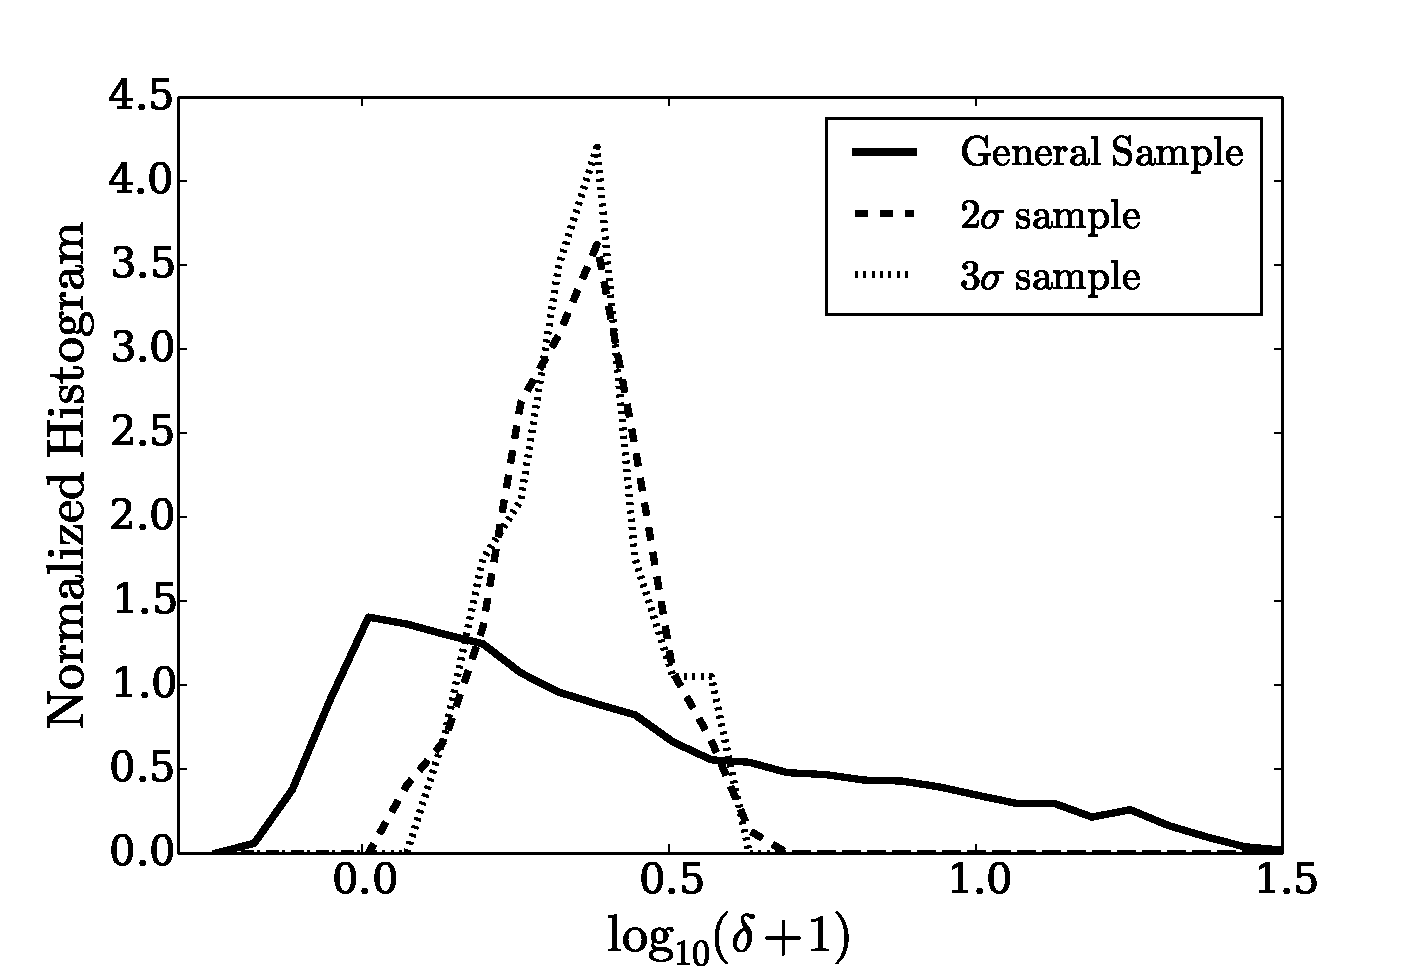
\includegraphics[width=0.50\textwidth]{density_histogram.pdf}
\end{center}
\caption{Overdensity distribution for the pairs in the three samples.
    \label{fig:density}}  
\end{figure}


In Figure \ref{fig:FA} we show the integrated distribution for the
Fractional Anisotropy in the tree samples. The General Sample clusters
towards values of ${\mathrm FA}\sim 1.0$, while the $2\sigma$ and
$3\sigma$ prefer values around $0.6$.

\begin{figure*}
\begin{center}
  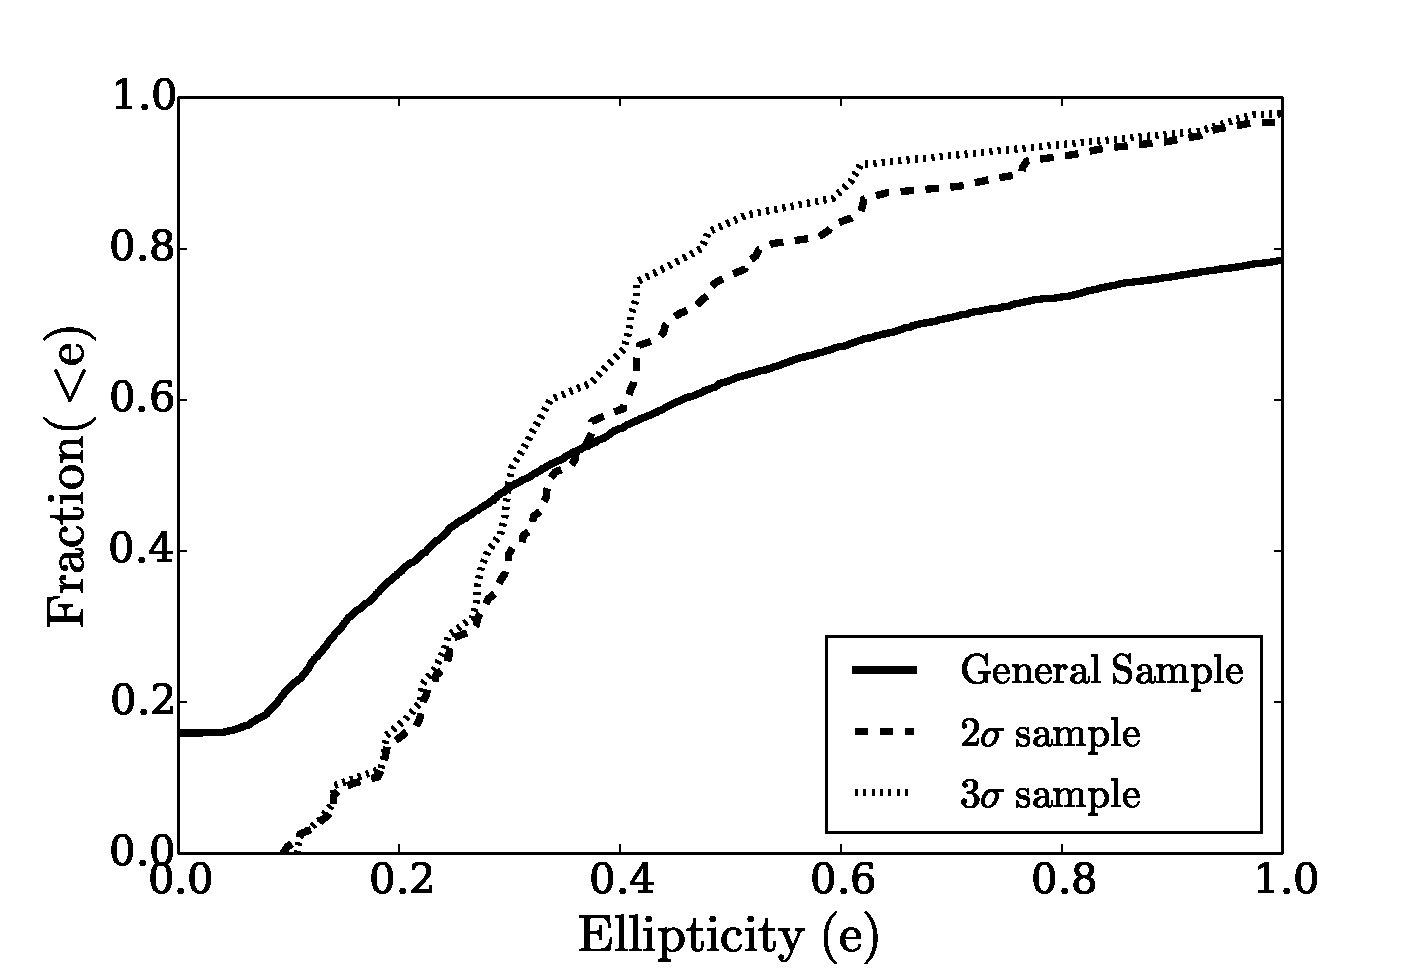
\includegraphics[width=0.49\textwidth]{ELL_histogram.pdf}
  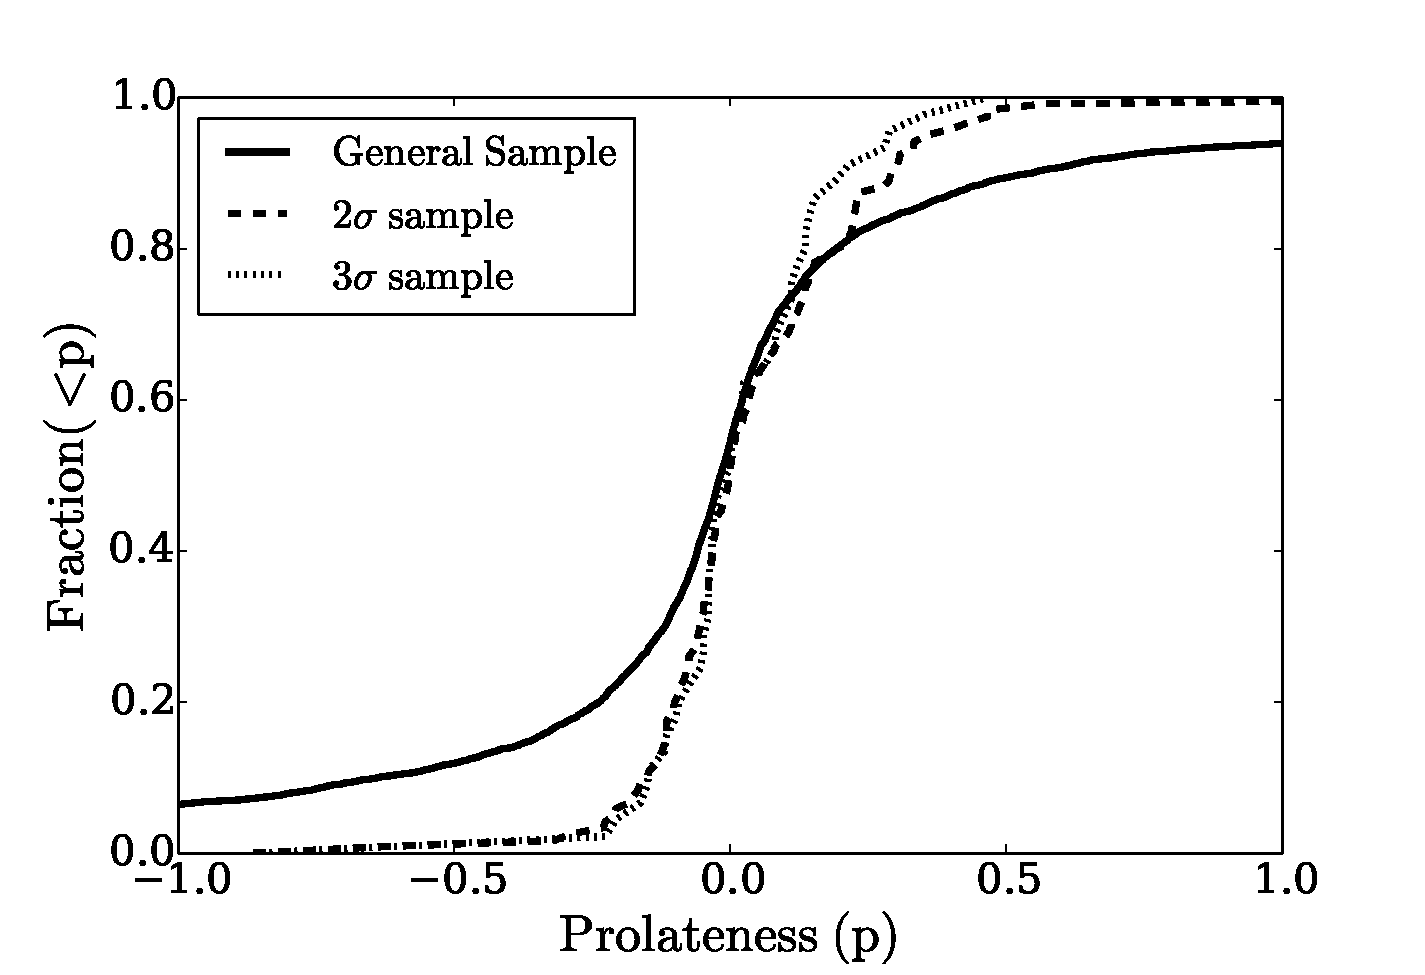
\includegraphics[width=0.49\textwidth]{PROL_histogram.pdf}
\end{center}
\caption{Cumulative distributions for the ellipticity and prolateness.
    \label{fig:ELL_PROL}}  
\end{figure*}

In Figure \ref{fig:delta_FA} we present a joint scatter plot for the
overdensity and fractional anisotropy. For clarity we only include the
general and $3\sigma$ samples. In this plane we observe from the general
sample that there are broad correlations between the overdensity and
the fractional anisotropy. 




\begin{figure*}
\begin{center}
  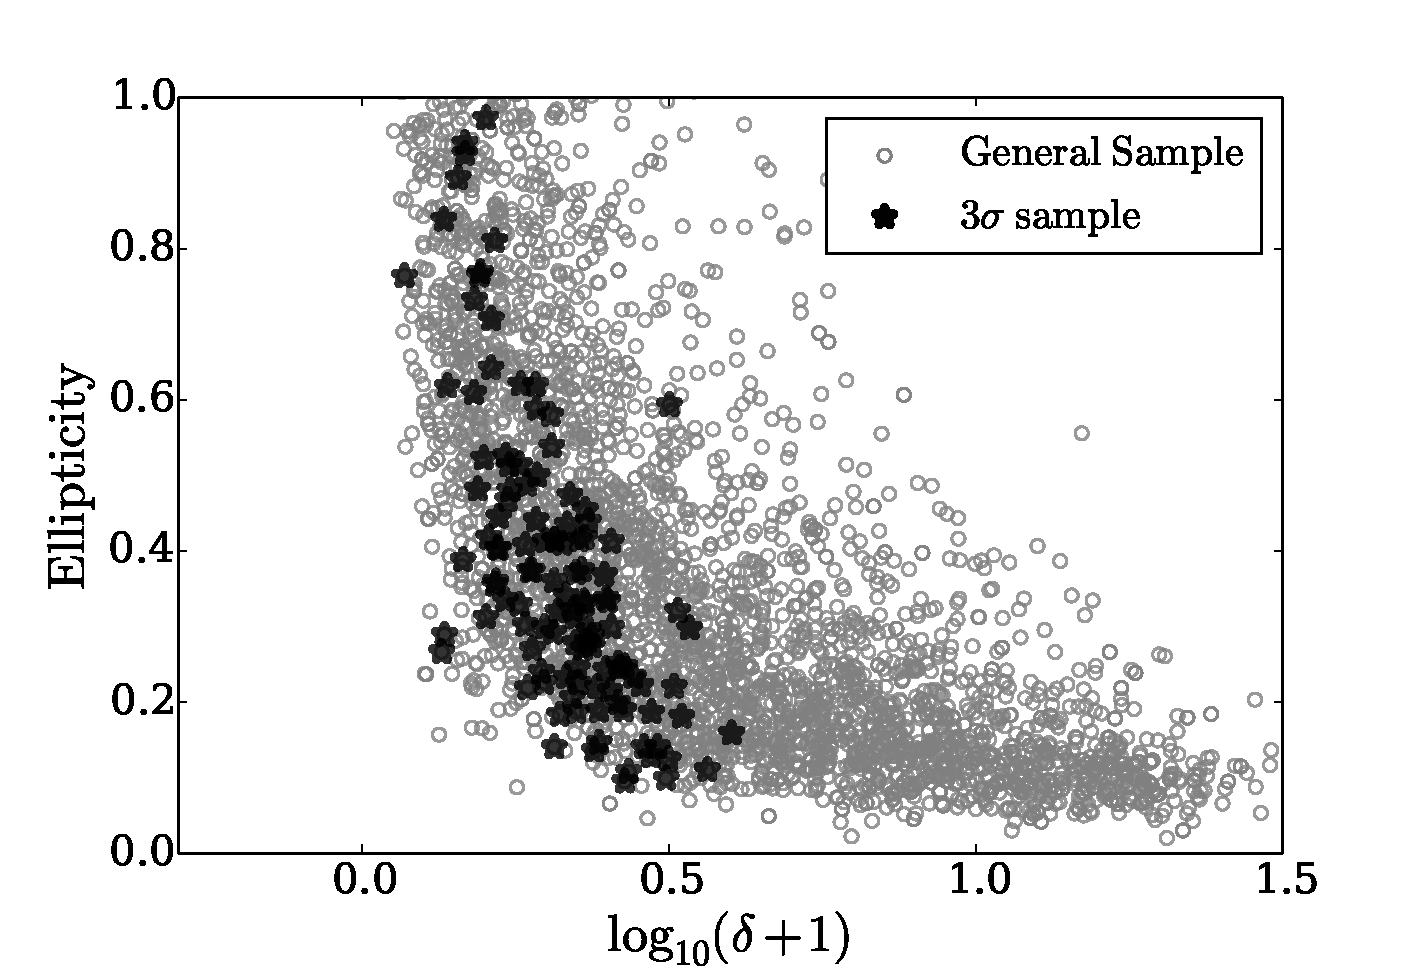
\includegraphics[width=0.49\textwidth]{ELL_delta_scatter.pdf}
  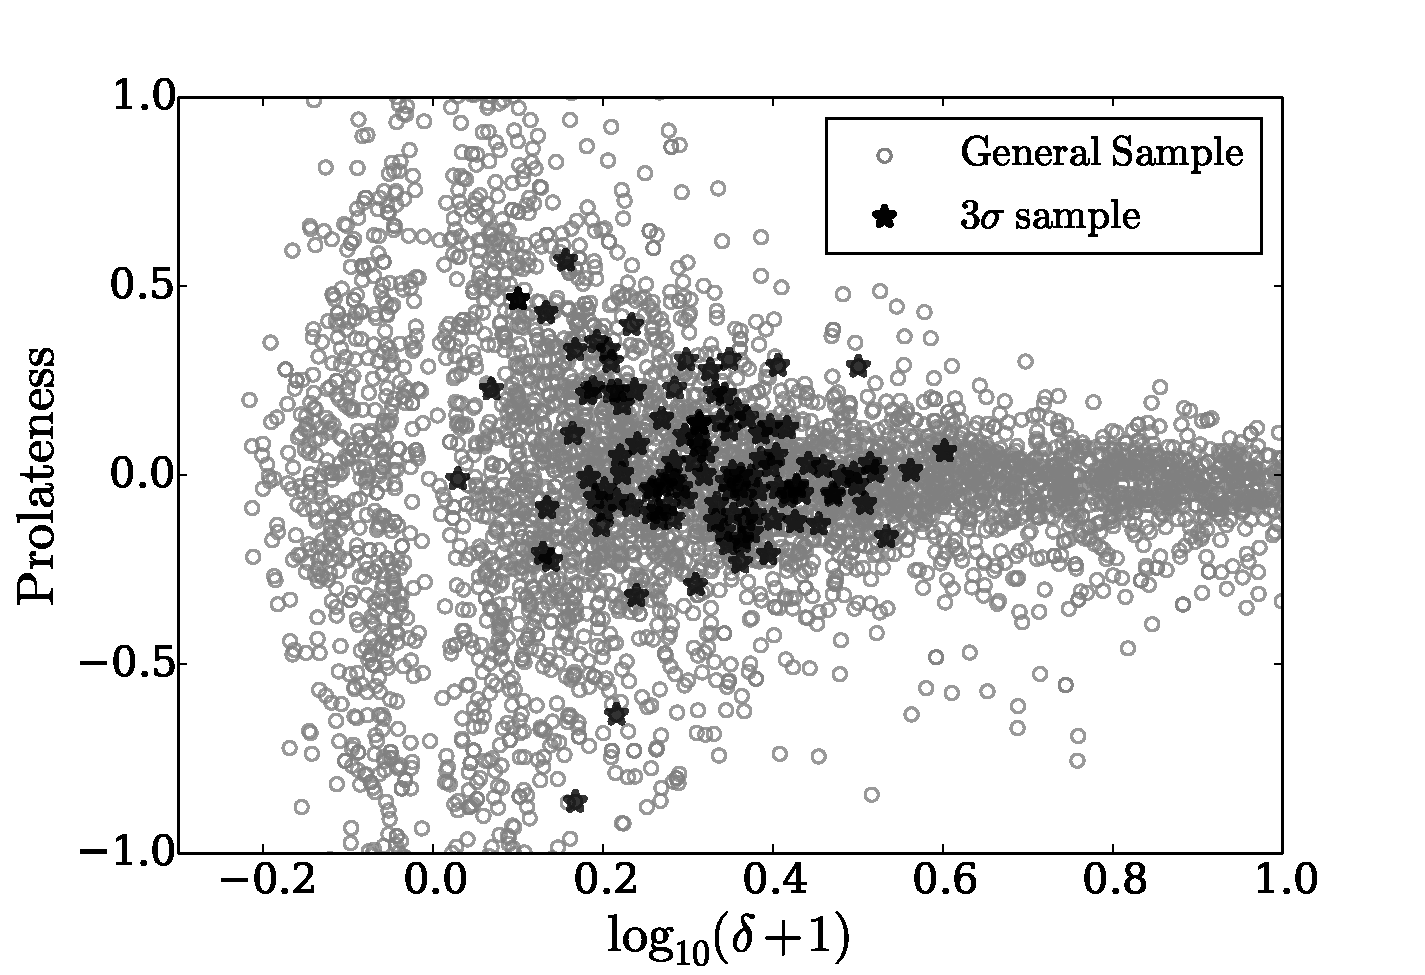
\includegraphics[width=0.49\textwidth]{PROL_delta_scatter.pdf}
\end{center}
\caption{Ellipticity and prolateness versus the overdensity for the pairs
  in the general and $3\sigma$ samples.  \label{fig:delta_ELL_PROL}}  
\end{figure*}


\begin{figure}
\begin{center}
  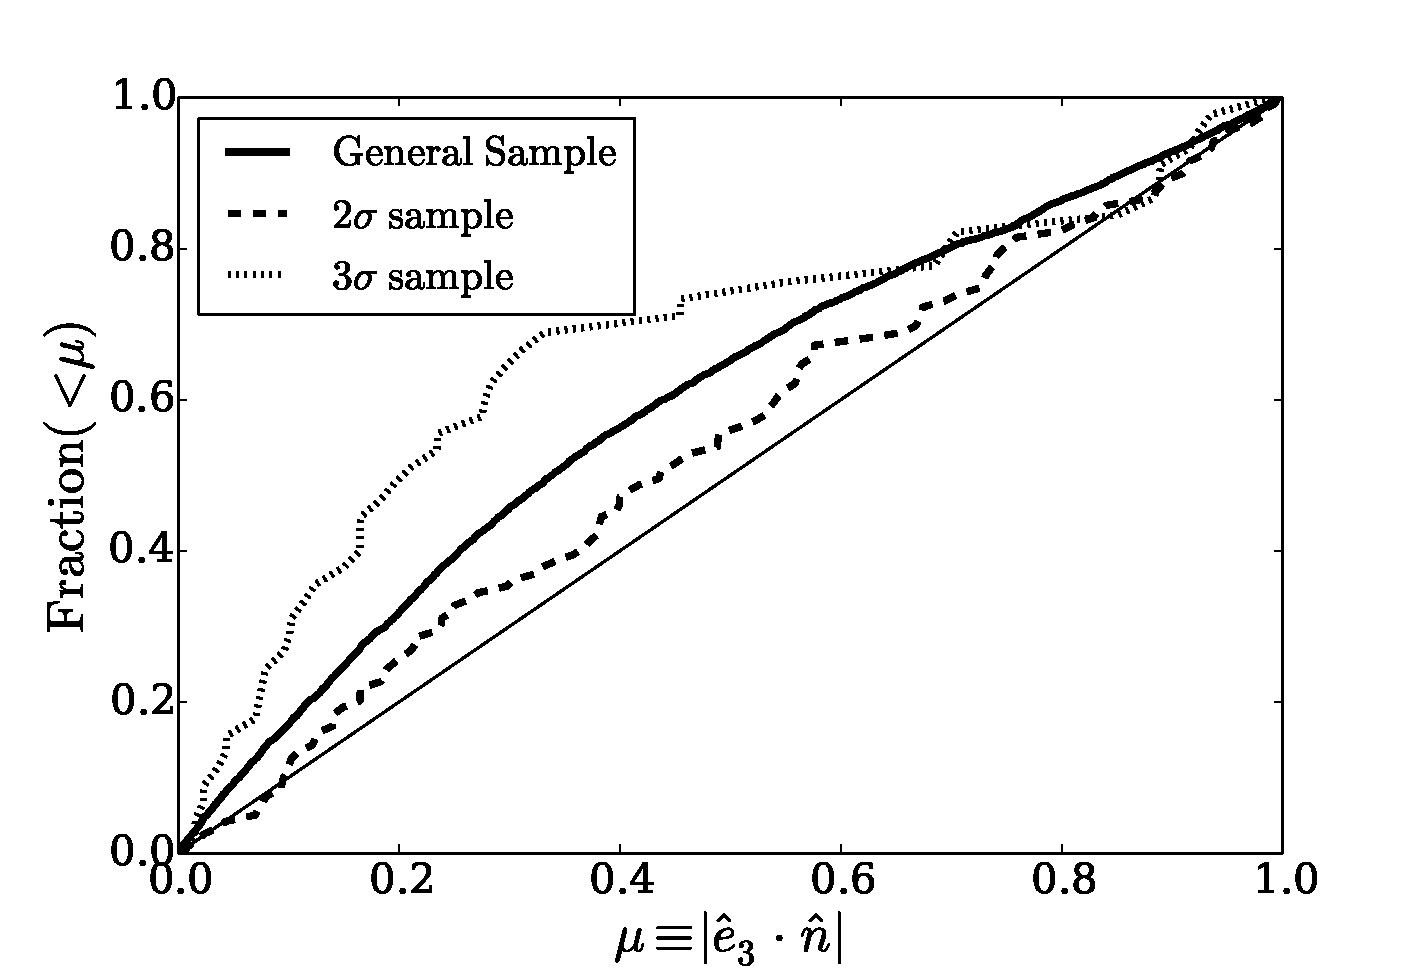
\includegraphics[width=0.50\textwidth]{alignments_e3.pdf} 
\end{center}
\caption{Cumulative distributions for the alignment between the normal
  vector $\hat{n}$ and the third eigenvector $\vec{e}_3$.
    \label{fig:alignment}}  
\end{figure}

\begin{table}
\begin{center}
\begin{tabular}{lccc}\hline\hline
Sample & $\langle\hat{e}_1\cdot \hat{n}\rangle$ & $\langle\hat{e}_2\cdot \hat{n}\rangle$ & $\langle\hat{e}_3\cdot \hat{n}\rangle$\\\hline
2$\sigma$ & 0.56 & 0.53 &  0.33\\
3$\sigma$ & 0.51 & 0.51 &  0.46\\
General & 0.54 & 0.52 & 0.40\\\hline
\end{tabular}
\caption{Average values for the cosinus between the three eigenvectors and the vector normal to the orbital plane.
\label{table:mu}}
\end{center}
\end{table}


\subsection{Alignment along the cosmic web}


\section{Discussion}
\label{sec:discussion}

\section{Conclusions}
\label{sec:conclusions}


\section*{Acknowledgements}

\bibliographystyle{apj}
\bibliography{references} 


\end{document}


